
%% 1-2 pages

\section{Related research}

This section presents and reviews the research from two main areas, technical debt management and information visualization, upon which this study builds.

\subsection{Technical Debt}
First described by Cunningham in 1992 \cite{cunningham_wycash_1992}, technical debt (TB) is a metaphor to financial debt and describes the common situation with increased development costs over time in software projects caused by poor software engineering practices \cite{tom_exploration_2013}.


\subsection{Information Visualization}

The core of information visualizations are the mapping of data and intent to visual representations.
Although there are many different techniques used in the field, this central process of visualizations can be described by the \textit{Reference model for visualization} by Card et al. presented in figure \ref{fig:vizprocess} \cite{card_readings_1999}. 
This common reference model is helpful in order to analyze and compare the different techniques as seen in the taxonomy proposed by Chi based on model by Card et al. \cite{chi_taxonomy_2000}.

\begin{figure}[t]
  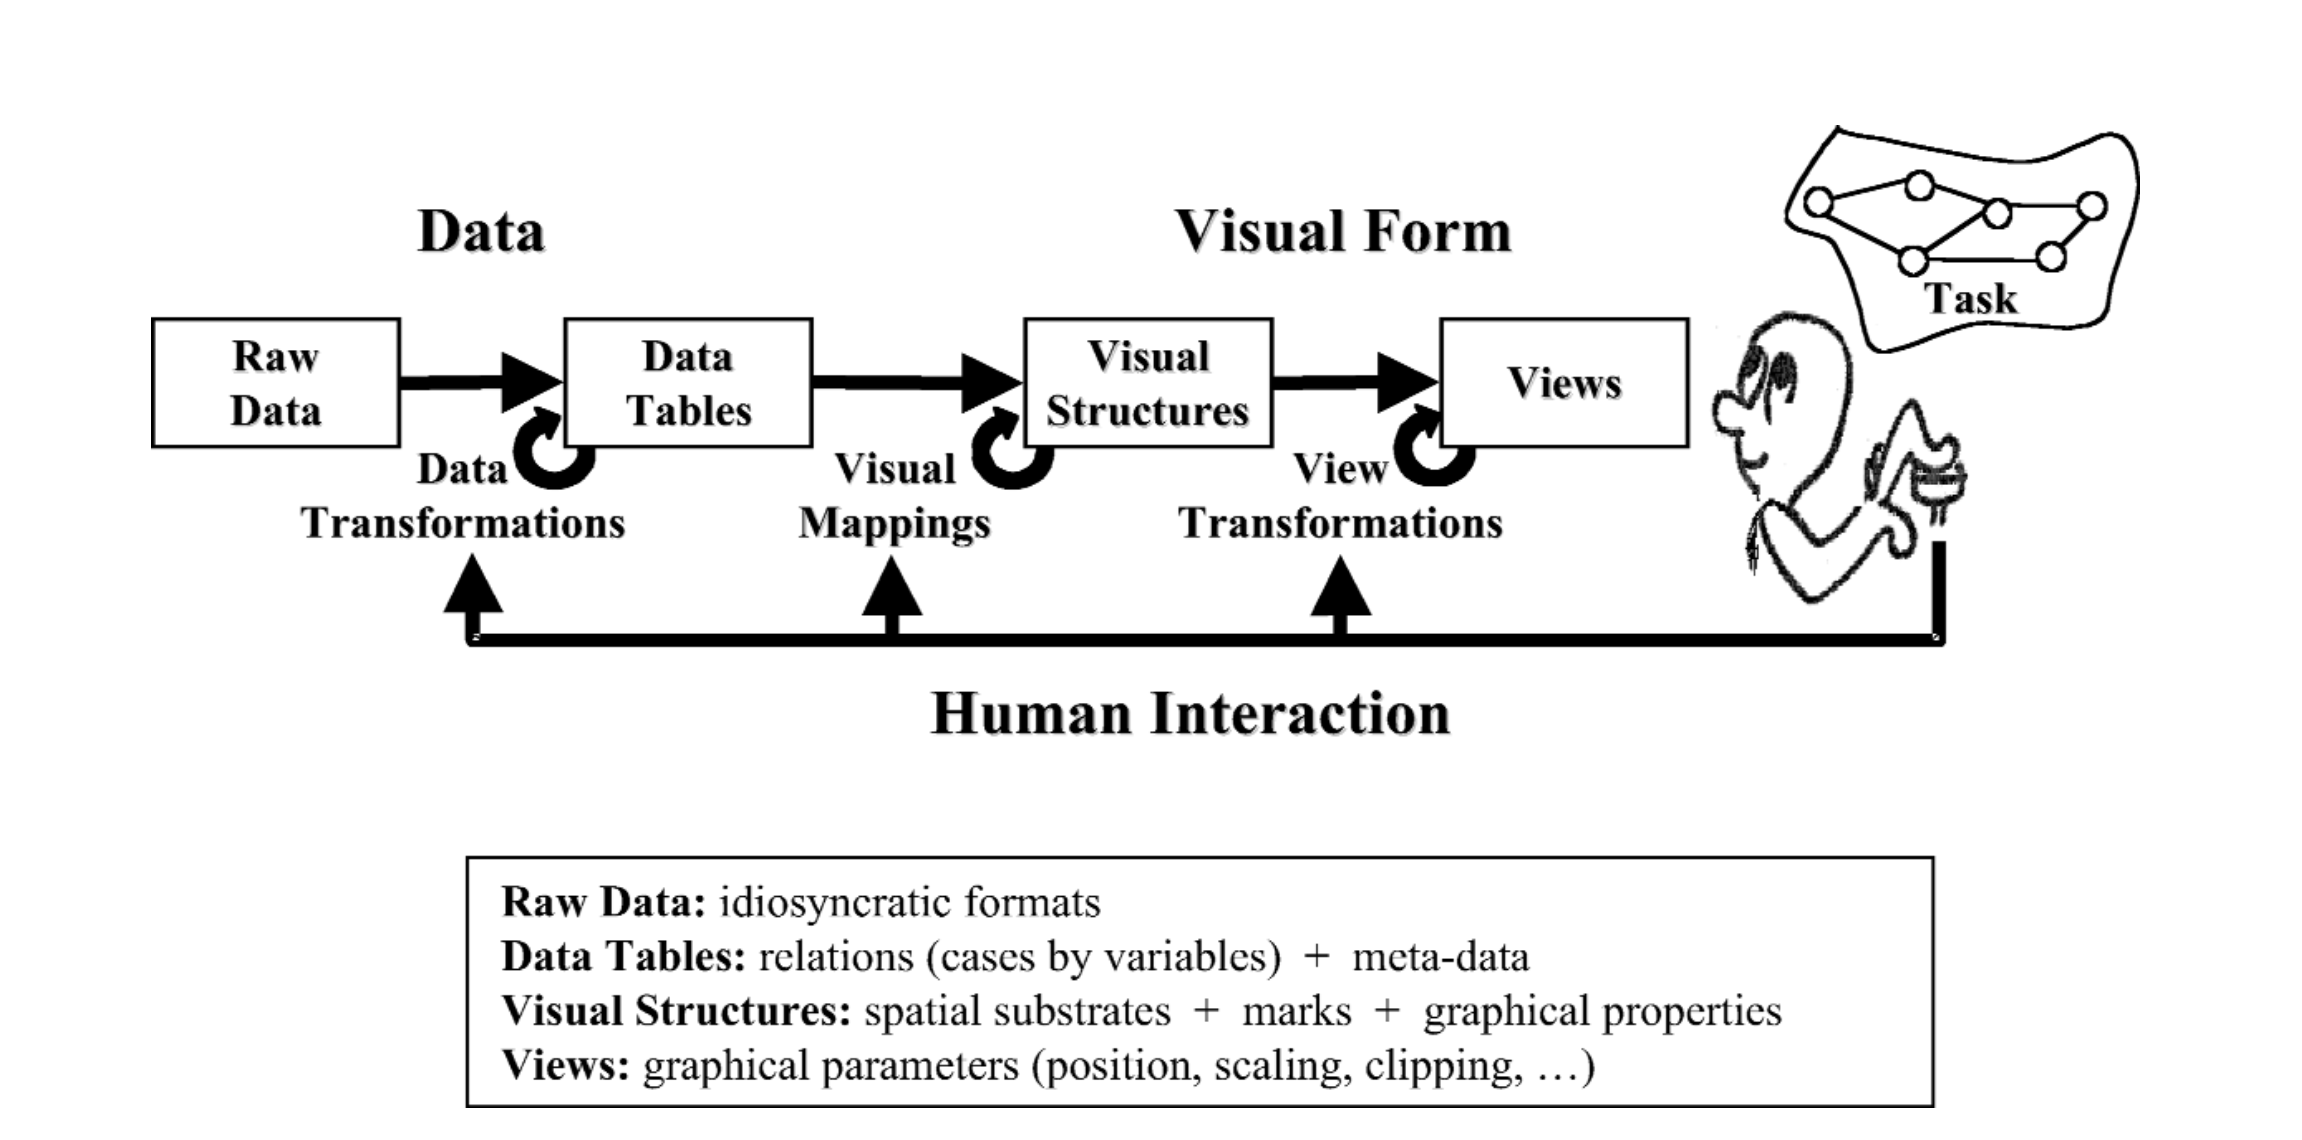
\includegraphics[width=\columnwidth]{VisualizationProcess}
  \Description{Chart over the Reference model for visualization by Card et al. 1999}
  \caption[Reference model for visualization]{Reference model for visualization by Card et al. 1999 \cite{card_readings_1999}}.
  \label{fig:vizprocess}
  \centering
\end{figure}

The raw data can take many forms which can be classified intro three main categories based on its properties, \textit{nominal data} is simple data with some sort of label but no quantitative value, \textit{ordinal data} can be ranked according to some attribute and \textit{quantitative data} which support arithmetic operations \cite{card_structure_1997}.
